% Created by tikzDevice version 0.12.3 on 2019-12-11 20:53:29
% !TEX encoding = UTF-8 Unicode
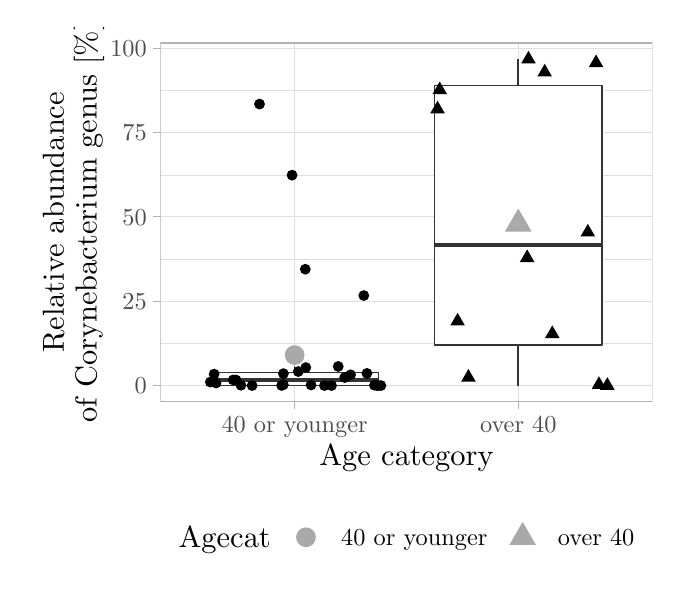
\begin{tikzpicture}[x=1pt,y=1pt]
\definecolor{fillColor}{RGB}{255,255,255}
\path[use as bounding box,fill=fillColor,fill opacity=0.00] (0,0) rectangle (231.26,202.36);
\begin{scope}
\path[clip] (  0.00,  0.00) rectangle (231.26,202.36);
\definecolor{drawColor}{RGB}{255,255,255}
\definecolor{fillColor}{RGB}{255,255,255}

\path[draw=drawColor,line width= 0.6pt,line join=round,line cap=round,fill=fillColor] (  0.00,  0.00) rectangle (231.26,202.36);
\end{scope}
\begin{scope}
\path[clip] ( 47.99, 67.14) rectangle (225.76,196.86);
\definecolor{fillColor}{RGB}{255,255,255}

\path[fill=fillColor] ( 47.99, 67.14) rectangle (225.76,196.86);
\definecolor{drawColor}{gray}{0.87}

\path[draw=drawColor,line width= 0.1pt,line join=round] ( 47.99, 88.28) --
	(225.76, 88.28);

\path[draw=drawColor,line width= 0.1pt,line join=round] ( 47.99,118.75) --
	(225.76,118.75);

\path[draw=drawColor,line width= 0.1pt,line join=round] ( 47.99,149.23) --
	(225.76,149.23);

\path[draw=drawColor,line width= 0.1pt,line join=round] ( 47.99,179.71) --
	(225.76,179.71);

\path[draw=drawColor,line width= 0.3pt,line join=round] ( 47.99, 73.04) --
	(225.76, 73.04);

\path[draw=drawColor,line width= 0.3pt,line join=round] ( 47.99,103.52) --
	(225.76,103.52);

\path[draw=drawColor,line width= 0.3pt,line join=round] ( 47.99,133.99) --
	(225.76,133.99);

\path[draw=drawColor,line width= 0.3pt,line join=round] ( 47.99,164.47) --
	(225.76,164.47);

\path[draw=drawColor,line width= 0.3pt,line join=round] ( 47.99,194.95) --
	(225.76,194.95);

\path[draw=drawColor,line width= 0.3pt,line join=round] ( 96.47, 67.14) --
	( 96.47,196.86);

\path[draw=drawColor,line width= 0.3pt,line join=round] (177.28, 67.14) --
	(177.28,196.86);

\path[] ( 96.47,115.07) circle (  1.96);

\path[] ( 96.47,105.56) circle (  1.96);

\path[] ( 96.47,149.06) circle (  1.96);

\path[] ( 96.47,174.75) circle (  1.96);
\definecolor{drawColor}{gray}{0.20}

\path[draw=drawColor,line width= 0.6pt,line join=round] ( 96.47, 77.77) -- ( 96.47, 79.94);

\path[draw=drawColor,line width= 0.6pt,line join=round] ( 96.47, 73.11) -- ( 96.47, 73.04);

\path[draw=drawColor,line width= 0.6pt,line join=round,line cap=round,fill=fillColor] ( 66.17, 77.77) --
	( 66.17, 73.11) --
	(126.78, 73.11) --
	(126.78, 77.77) --
	( 66.17, 77.77) --
	cycle;

\path[draw=drawColor,line width= 1.1pt,line join=round] ( 66.17, 75.04) -- (126.78, 75.04);

\path[draw=drawColor,line width= 0.6pt,line join=round] (177.28,181.45) -- (177.28,190.96);

\path[draw=drawColor,line width= 0.6pt,line join=round] (177.28, 87.78) -- (177.28, 73.04);

\path[draw=drawColor,line width= 0.6pt,line join=round,line cap=round,fill=fillColor] (146.98,181.45) --
	(146.98, 87.78) --
	(207.58, 87.78) --
	(207.58,181.45) --
	(146.98,181.45) --
	cycle;

\path[draw=drawColor,line width= 1.1pt,line join=round] (146.98,123.82) -- (207.58,123.82);
\definecolor{fillColor}{RGB}{0,0,0}

\path[fill=fillColor] (114.56, 75.94) circle (  1.96);

\path[fill=fillColor] (127.64, 73.04) circle (  1.96);

\path[fill=fillColor] (100.50, 79.54) circle (  1.96);

\path[fill=fillColor] (109.80, 73.04) circle (  1.96);

\path[fill=fillColor] (205.39,192.66) --
	(208.03,188.08) --
	(202.74,188.08) --
	cycle;

\path[fill=fillColor] ( 81.10, 73.04) circle (  1.96);

\path[fill=fillColor] (100.32,115.07) circle (  1.96);

\path[fill=fillColor] ( 68.06, 73.96) circle (  1.96);

\path[fill=fillColor] (148.10,175.97) --
	(150.75,171.39) --
	(145.46,171.39) --
	cycle;

\path[fill=fillColor] (180.48,122.25) --
	(183.12,117.68) --
	(177.84,117.68) --
	cycle;

\path[fill=fillColor] (209.46, 76.09) --
	(212.10, 71.51) --
	(206.82, 71.51) --
	cycle;

\path[fill=fillColor] (159.27, 79.03) --
	(161.92, 74.45) --
	(156.63, 74.45) --
	cycle;

\path[fill=fillColor] (186.82,189.31) --
	(189.46,184.73) --
	(184.18,184.73) --
	cycle;

\path[fill=fillColor] ( 75.31, 75.04) circle (  1.96);

\path[fill=fillColor] (155.35, 99.33) --
	(157.99, 94.75) --
	(152.70, 94.75) --
	cycle;

\path[fill=fillColor] (121.46,105.56) circle (  1.96);

\path[fill=fillColor] ( 74.29, 75.07) circle (  1.96);

\path[fill=fillColor] (122.59, 77.44) circle (  1.96);

\path[fill=fillColor] ( 77.06, 73.15) circle (  1.96);

\path[fill=fillColor] ( 97.78, 78.10) circle (  1.96);

\path[fill=fillColor] (125.31, 73.15) circle (  1.96);

\path[fill=fillColor] (189.57, 94.77) --
	(192.22, 90.19) --
	(186.93, 90.19) --
	cycle;

\path[fill=fillColor] (112.21, 79.94) circle (  1.96);

\path[fill=fillColor] (202.41,131.48) --
	(205.05,126.90) --
	(199.76,126.90) --
	cycle;

\path[fill=fillColor] ( 91.77, 73.07) circle (  1.96);

\path[fill=fillColor] (148.89,182.90) --
	(151.53,178.33) --
	(146.25,178.33) --
	cycle;

\path[fill=fillColor] (126.57, 73.04) circle (  1.96);

\path[fill=fillColor] (206.44, 76.40) --
	(209.08, 71.82) --
	(203.80, 71.82) --
	cycle;

\path[fill=fillColor] (102.39, 73.26) circle (  1.96);

\path[fill=fillColor] ( 95.54,149.06) circle (  1.96);

\path[fill=fillColor] (180.96,194.01) --
	(183.60,189.43) --
	(178.32,189.43) --
	cycle;

\path[fill=fillColor] ( 83.78,174.75) circle (  1.96);

\path[fill=fillColor] (126.32, 73.04) circle (  1.96);

\path[fill=fillColor] ( 67.38, 77.17) circle (  1.96);

\path[fill=fillColor] (116.68, 76.92) circle (  1.96);

\path[fill=fillColor] (107.24, 73.04) circle (  1.96);

\path[fill=fillColor] ( 66.01, 74.29) circle (  1.96);

\path[fill=fillColor] ( 92.41, 77.35) circle (  1.96);

\path[fill=fillColor] ( 92.38, 73.37) circle (  1.96);
\definecolor{fillColor}{RGB}{169,169,169}

\path[fill=fillColor] ( 96.47, 84.05) circle (  3.57);

\path[fill=fillColor] (177.28,137.01) --
	(182.09,128.69) --
	(172.47,128.69) --
	cycle;
\definecolor{drawColor}{gray}{0.70}

\path[draw=drawColor,line width= 0.6pt,line join=round,line cap=round] ( 47.99, 67.14) rectangle (225.76,196.86);
\end{scope}
\begin{scope}
\path[clip] (  0.00,  0.00) rectangle (231.26,202.36);
\definecolor{drawColor}{gray}{0.30}

\node[text=drawColor,anchor=base east,inner sep=0pt, outer sep=0pt, scale=  0.88] at ( 43.04, 70.01) {0};

\node[text=drawColor,anchor=base east,inner sep=0pt, outer sep=0pt, scale=  0.88] at ( 43.04,100.48) {25};

\node[text=drawColor,anchor=base east,inner sep=0pt, outer sep=0pt, scale=  0.88] at ( 43.04,130.96) {50};

\node[text=drawColor,anchor=base east,inner sep=0pt, outer sep=0pt, scale=  0.88] at ( 43.04,161.44) {75};

\node[text=drawColor,anchor=base east,inner sep=0pt, outer sep=0pt, scale=  0.88] at ( 43.04,191.92) {100};
\end{scope}
\begin{scope}
\path[clip] (  0.00,  0.00) rectangle (231.26,202.36);
\definecolor{drawColor}{gray}{0.70}

\path[draw=drawColor,line width= 0.3pt,line join=round] ( 45.24, 73.04) --
	( 47.99, 73.04);

\path[draw=drawColor,line width= 0.3pt,line join=round] ( 45.24,103.52) --
	( 47.99,103.52);

\path[draw=drawColor,line width= 0.3pt,line join=round] ( 45.24,133.99) --
	( 47.99,133.99);

\path[draw=drawColor,line width= 0.3pt,line join=round] ( 45.24,164.47) --
	( 47.99,164.47);

\path[draw=drawColor,line width= 0.3pt,line join=round] ( 45.24,194.95) --
	( 47.99,194.95);
\end{scope}
\begin{scope}
\path[clip] (  0.00,  0.00) rectangle (231.26,202.36);
\definecolor{drawColor}{gray}{0.70}

\path[draw=drawColor,line width= 0.3pt,line join=round] ( 96.47, 64.39) --
	( 96.47, 67.14);

\path[draw=drawColor,line width= 0.3pt,line join=round] (177.28, 64.39) --
	(177.28, 67.14);
\end{scope}
\begin{scope}
\path[clip] (  0.00,  0.00) rectangle (231.26,202.36);
\definecolor{drawColor}{gray}{0.30}

\node[text=drawColor,anchor=base,inner sep=0pt, outer sep=0pt, scale=  0.88] at ( 96.47, 56.13) {40 or younger};

\node[text=drawColor,anchor=base,inner sep=0pt, outer sep=0pt, scale=  0.88] at (177.28, 56.13) {over 40};
\end{scope}
\begin{scope}
\path[clip] (  0.00,  0.00) rectangle (231.26,202.36);
\definecolor{drawColor}{RGB}{0,0,0}

\node[text=drawColor,anchor=base,inner sep=0pt, outer sep=0pt, scale=  1.10] at (136.88, 44.09) {Age category};
\end{scope}
\begin{scope}
\path[clip] (  0.00,  0.00) rectangle (231.26,202.36);
\definecolor{drawColor}{RGB}{0,0,0}

\node[text=drawColor,rotate= 90.00,anchor=base,inner sep=0pt, outer sep=0pt, scale=  1.10] at ( 13.08,132.00) {Relative abundance };

\node[text=drawColor,rotate= 90.00,anchor=base,inner sep=0pt, outer sep=0pt, scale=  1.10] at ( 24.96,132.00) { of Corynebacterium genus [\%]};
\end{scope}
\begin{scope}
\path[clip] (  0.00,  0.00) rectangle (231.26,202.36);
\definecolor{fillColor}{RGB}{255,255,255}

\path[fill=fillColor] ( 49.04,  5.50) rectangle (224.72, 30.95);
\end{scope}
\begin{scope}
\path[clip] (  0.00,  0.00) rectangle (231.26,202.36);
\definecolor{drawColor}{RGB}{0,0,0}

\node[text=drawColor,anchor=base west,inner sep=0pt, outer sep=0pt, scale=  1.10] at ( 54.54, 14.44) {Agecat};
\end{scope}
\begin{scope}
\path[clip] (  0.00,  0.00) rectangle (231.26,202.36);
\definecolor{fillColor}{RGB}{255,255,255}

\path[fill=fillColor] ( 93.33, 11.00) rectangle (107.79, 25.45);
\end{scope}
\begin{scope}
\path[clip] (  0.00,  0.00) rectangle (231.26,202.36);
\definecolor{fillColor}{RGB}{0,0,0}

\path[fill=fillColor] (100.56, 18.23) circle (  1.96);
\end{scope}
\begin{scope}
\path[clip] (  0.00,  0.00) rectangle (231.26,202.36);
\definecolor{fillColor}{RGB}{169,169,169}

\path[fill=fillColor] (100.56, 18.23) circle (  3.57);
\end{scope}
\begin{scope}
\path[clip] (  0.00,  0.00) rectangle (231.26,202.36);
\definecolor{fillColor}{RGB}{255,255,255}

\path[fill=fillColor] (171.62, 11.00) rectangle (186.08, 25.45);
\end{scope}
\begin{scope}
\path[clip] (  0.00,  0.00) rectangle (231.26,202.36);
\definecolor{fillColor}{RGB}{0,0,0}

\path[fill=fillColor] (178.85, 21.28) --
	(181.49, 16.70) --
	(176.21, 16.70) --
	cycle;
\end{scope}
\begin{scope}
\path[clip] (  0.00,  0.00) rectangle (231.26,202.36);
\definecolor{fillColor}{RGB}{169,169,169}

\path[fill=fillColor] (178.85, 23.78) --
	(183.66, 15.45) --
	(174.05, 15.45) --
	cycle;
\end{scope}
\begin{scope}
\path[clip] (  0.00,  0.00) rectangle (231.26,202.36);
\definecolor{drawColor}{RGB}{0,0,0}

\node[text=drawColor,anchor=base west,inner sep=0pt, outer sep=0pt, scale=  0.88] at (113.29, 15.20) {40 or younger};
\end{scope}
\begin{scope}
\path[clip] (  0.00,  0.00) rectangle (231.26,202.36);
\definecolor{drawColor}{RGB}{0,0,0}

\node[text=drawColor,anchor=base west,inner sep=0pt, outer sep=0pt, scale=  0.88] at (191.58, 15.20) {over 40};
\end{scope}
\end{tikzpicture}
